
\documentclass[12pt,a4paper,oneside]{report}

\usepackage[T1]{fontenc}
\usepackage{times}
\usepackage[utf8]{inputenc}
\usepackage{amsmath}
\usepackage{graphicx}
\usepackage{multicol}
\usepackage{longtable}
\usepackage[refpages]{gloss}
\usepackage{float}
\usepackage{anysize}
\usepackage{appendix}
\usepackage{lscape} 
\usepackage{pdflscape}
\usepackage{multirow}
\usepackage{listings}
\usepackage{color}
\usepackage{setspace}
\usepackage{enumerate} 
\usepackage{natbib}
\usepackage{graphicx}
\usepackage[utf8]{inputenc}
 
\usepackage{listings}
\usepackage{color}
 
\definecolor{codegreen}{rgb}{0,0.6,0}
\definecolor{codegray}{rgb}{0.5,0.5,0.5}
\definecolor{codepurple}{rgb}{0.58,0,0.82}
\definecolor{backcolour}{rgb}{0.95,0.95,0.92}
 
\lstdefinestyle{mystyle}{
    backgroundcolor=\color{backcolour},   
    commentstyle=\color{codegreen},
    keywordstyle=\color{magenta},
    numberstyle=\tiny\color{codegray},
    stringstyle=\color{codepurple},
    basicstyle=\footnotesize,
    breakatwhitespace=false,         
    breaklines=true,                 
    captionpos=b,                    
    keepspaces=true,                 
    numbers=left,                    
    numbersep=5pt,                  
    showspaces=false,                
    showstringspaces=false,
    showtabs=false,                  
    tabsize=2
}
 
\lstset{style=mystyle}
 


\begin{document}

\marginsize{3.0cm}{3.0cm}{4.0cm}{3.0cm}
\renewcommand*{\contentsname}{Problem}
\begin{titlepage}
 
\begin{center}
 
 {\huge \bf EE1390}\\
 
{\Large Intro to AI and ML}\\[2.0cm]


\begin{center}

\includegraphics[width=0.4\textwidth]{imagenes/iith.png}
\end{center}

\vspace{1cm}
\title{} 
{\bf \large . }\\[1cm] 
{{\bf Autor}: me17btech11037 - me17btech11040 }\\[2.0cm] 
{\large Vijay and surya}\\[0.2cm] 
{assignment 1}
\end{center}

\end{titlepage}
\chapter*{\centering \large 22. If an equlateral triangle, having centroid at the
origin, has \ a \ side \ along \ the \ line \ (1 1) x = 2,then \ find \ the \ area  \ of \ this \ triangle.} 
\begin{figure}[h!]
\centering
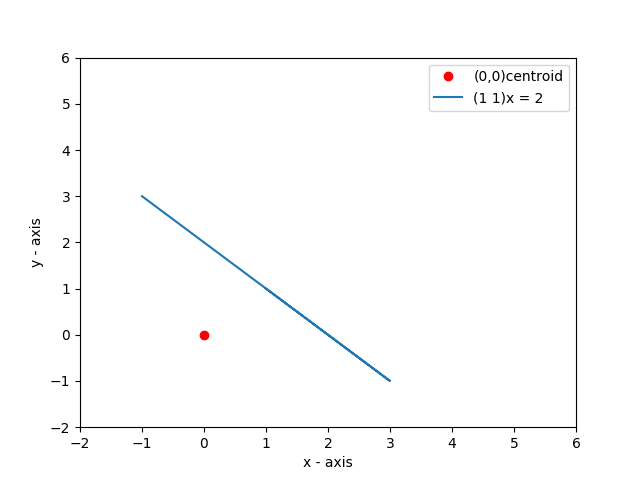
\includegraphics[scale=0.9]{imagenes/question.png}
\caption{Given question}
\label{fig:question}
\end{figure}
{\Large Solution: } \\[5.00mm]
{\      Given centroid\\
$
O = \begin{pmatrix} 0 & 0 \end{pmatrix} \\
 M = \begin{pmatrix} 1 & 1 \end{pmatrix} \\
 M^{-1} = \begin{pmatrix} 1 & 1 \end{pmatrix}\begin{pmatrix} 0 & 1 \\ -1 & 0 \end{pmatrix} = \begin{pmatrix} -1 & 1 \end{pmatrix}
 slope \ of\  perpendicular\ of \ the\ given\ line\\
 S =\begin{pmatrix} 1 & 1 \\ -1 & 1 \end{pmatrix}\\ [2.00mm]
 finding \ point \ of \ intersection\ of\ perpendicular \ and \ given \ line\\[2.00mm]
 D =\begin{pmatrix} 2 & 0 \end{pmatrix}\\
 S.X{^T} = D{^T} \ for\ finding \ the\ point\ of\ intersection\\[2.00mm]
 length \ of\ \bot \ from \ circumcenter  \ d = X - O \\ [2.00mm]
 v =  \sqrt{d.d^{T}} \\ where \ v \ is \ the \ distance \\[2.00mm]
 length \ of \ the \ equalateral \ triangle \\ = 3\ * v *sin(60)
 area = 0.5*length*length*sin(60)
 $\\[5.00mm]
 points can be  relocated using \\
 $ B =X +(length* M_inv)/2 \\
 C= X-(length* M_inv)/2 $}\\[5.00mm]
 
 {\Large Output figure}
\begin{figure}[h!]
\centering
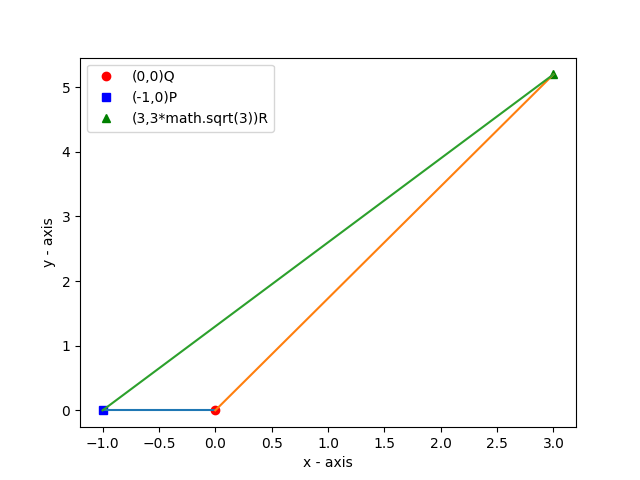
\includegraphics[scale=1]{imagenes/Figure_1.png}
\caption{Obtained graph}
\label{fig:graph}
\end{figure}

\begin{lstlisting}[language=Python, caption=Python program  ]
#program to calculate area of an equalateraltraiangle given centroid and line equation

import numpy as np
import matplotlib.pyplot as plt
             #given condition

#ploting for solution


c=2
O = np.array([[0,0]]) #centroid
M = np.array([[1,1]])
inv = np.array([[0,1],[-1,0]])
M_inv = np.matmul(M,inv) #finding inverse
S = np.concatenate((M, M_inv))
e = M_inv*O.T
f = e[0,0]
D = np.array([c,f])
X = np.matmul(D,np.linalg.inv(S).T)
d = X - O
v = np.linalg.norm(d)
length = 3*v/(np.sin(np.pi/3))
area = 0.5*length*length*np.sin(np.pi/3)
v = np.linalg.norm(M)
M=M/v
B = X+(length*M_inv)/2 #locating points B and C
C = X-(length*M_inv)/2
A = 3*O - 2*X
print(area)
#plotting triangle
Q = np.array([A[0,0],A[0,1]])
A = Q
Q = np.array([B[0,0],B[0,1]])
B = Q
Q = np.array([C[0,0],C[0,1]])
C = Q

len =10

lam_1 = np.linspace(0,1,len)

x_AB = np.zeros((2,len))
x_BC = np.zeros((2,len))
x_CA = np.zeros((2,len))
for i in range(len):
    temp1 = A + lam_1[i]*(B-A)
    x_AB[:,i]= temp1.T
    temp2 = B + lam_1[i]*(C-B)
    x_BC[:,i]= temp2.T
    temp3 = C + lam_1[i]*(A-C)
    x_CA[:,i]= temp3.T
#print(x_AB[0,:],x_AB[1,:])
plt.plot(x_AB[0,:],x_AB[1,:],label='$AB$')
plt.plot(x_BC[0,:],x_BC[1,:],label='$BC$')
plt.plot(x_CA[0,:],x_CA[1,:],label='$CA$')

plt.plot(A[0], A[1], 'o')
plt.text(A[0] * (1 + 0.1), A[1] * (1 - 0.1) , 'A')
plt.plot(B[0], B[1], 'o')
plt.text(B[0] * (1 - 0.2), B[1] * (1) , 'B')
plt.plot(C[0], C[1], 'o')
plt.text(C[0] * (1 + 0.03), C[1] * (1 - 0.1) ,'C')

plt.xlabel('$x$')
plt.ylabel('$y$')
plt.legend(loc='best')
plt.grid() #minor

#else
plt.show()
\end{lstlisting}
\end{document} 


